%----------------------------------------------------------------------------------------
%	PACKAGES AND OTHER DOCUMENT CONFIGURATIONS
%----------------------------------------------------------------------------------------

\documentclass[12pt]{article}

\usepackage{polski}
\usepackage{ucs}
\usepackage[polish]{babel}
\usepackage[utf8x]{inputenc}
\usepackage{datetime}
\usepackage{graphicx}
\usepackage{color} 
\usepackage{tikz}
\usepackage{amsmath}
\usepackage{amsfonts}
\usepackage{epstopdf}
\usepackage{multirow}
\usepackage{tabularx}
\usepackage{listings} 
\usepackage{geometry}
 \geometry{
 	a4paper, 
 	left	=20mm,
 	right	=20mm,
 	top		=20mm,
 	bottom	=20mm,
 }
 
\definecolor{codegreen}{rgb}{0,0.6,0}
\definecolor{codegray}{rgb}{0.5,0.5,0.5}
\definecolor{codepurple}{rgb}{0.58,0,0.82}
\definecolor{backcolour}{rgb}{0.95,0.95,0.92}
 
\lstdefinestyle{mystyle}{
    backgroundcolor=\color{backcolour},   
    commentstyle=\color{codegreen},
    keywordstyle=\color{magenta},
    numberstyle=\tiny\color{codegray},
    stringstyle=\color{codepurple},
    basicstyle=\small,
    breakatwhitespace=false,         
    breaklines=true,                 
    captionpos=b,                    
    keepspaces=true,                 
    numbers=left,                    
    numbersep=5pt,                  
    showspaces=false,                
    showstringspaces=false,
    showtabs=false,                  
    tabsize=2  
}

\lstset{
    language=MATLAB,
    inputencoding=utf8x, 
    extendedchars=\true,
    basicstyle=\scriptsize,
    literate=
            {ą}{{\k{a}}}1
            {Ą}{{\k{A}}}1
            {ę}{{\k{e}}}1
            {Ę}{{\k{E}}}1
            {ó}{{\'o}}1
            {Ó}{{\'O}}1
            {ś}{{\'s}}1
            {Ś}{{\'S}}1
            {ł}{{\l{}}}1
            {Ł}{{\L{}}}1
            {ż}{{\.z}}1
            {Ż}{{\.Z}}1
            {ź}{{\'z}}1
            {Ź}{{\'Z}}1
            {ć}{{\'c}}1
            {Ć}{{\'C}}1
            {ń}{{\'n}}1
            {Ń}{{\'N}}1
}
 
%----------------------------------------------------------------------------------------
 
%----------------------------------------------------------------------------------------
% DATES
%----------------------------------------------------------------------------------------

\renewcommand{\dateseparator}{.}
\newdate{exercise_date}{20}{05}{2015}

%----------------------------------------------------------------------------------------

%----------------------------------------------------------------------------------------
% TIKZ PACKAGES
%----------------------------------------------------------------------------------------

\usetikzlibrary{arrows}

%----------------------------------------------------------------------------------------

\begin{document}
 
\begin{titlepage}

\newcommand{\HRule}{\rule{\linewidth}{0.5mm}}
% Defines a new command for the horizontal lines, change thickness here

\center
% Center everything on the page
 
%----------------------------------------------------------------------------------------
%	LOGO SECTION
%----------------------------------------------------------------------------------------


\includegraphics[width=6cm]{../res/img/logo.png}\\[1cm]
% Include a department/university logo - this will require the graphicx package
 
%----------------------------------------------------------------------------------------
 
%----------------------------------------------------------------------------------------
%	HEADING SECTIONS
%----------------------------------------------------------------------------------------

\textsc{\LARGE Akademia Górniczo-Hutnicza \\[0.2cm]
im. Stanisława Staszica w Krakowie}\\[1.5cm]
% Name of your university/college

\textsc{\Large Podstawy Automatyki}\\[0.5cm]
% Major heading such as course name

%----------------------------------------------------------------------------------------
%	TITLE SECTION
%----------------------------------------------------------------------------------------

\HRule \\[0.5cm]
{ \huge \bfseries Dyskretne układy regulacji \\[0.3cm] oraz \\[0.5cm] Analiza
serwomechanizmu \\[0.2cm] przekaźnikowego z wykorzystaniem płaszczyzny
fazowej}\\[0.3cm]
% Title of your document
\HRule \\[1.5cm]
 
%----------------------------------------------------------------------------------------
%	AUTHOR SECTION
%----------------------------------------------------------------------------------------

% \begin{minipage}{0.4\textwidth}
% \begin{flushleft} \large
% \emph{Author:}\\
% Konrad \textsc{Adasiewcz} % Your name
% \end{flushleft}
% \end{minipage}
% ~
% \begin{minipage}{0.4\textwidth}
% \begin{flushright} \large
% \emph{Supervisor:} \\
% dr inż. Paweł \textsc{Rotter} % Supervisor's Name
% \end{flushright}
% \end{minipage}\\[4cm]

% If you don't want a supervisor, uncomment the two lines below and remove the section above
\flushright
\Large \emph{Autorzy:}\\
Konrad \textsc{Adasiewcz}\\[0.1cm] % Your name
Michał \textsc{Maciejewski}\\[3cm] % Your name

%----------------------------------------------------------------------------------------
%	DATE SECTION
%----------------------------------------------------------------------------------------
Data wykonania ćwiczenia: \\
{\large \displaydate{exercise_date}}\\[1cm]


\vfill % Fill the rest of the page with whitespace

\end{titlepage}

\section*{Wstęp}

Przed autorem został postawiony problem stworzenia aplikacji w pakiecie
\textsc{Matlab}, implementaującej algorytm największego spadku
do poszukiwania minimum funkcjonału, na przykładzie funkcji benchmarkowej
Rosenbrocka w wersji dziesięcowymiarowej.
Dodatkowym założeniem dla projektowanej aplikacji była maksymalna elastyczność w
postaci prostej podmiany minimalizowanej funkcji czy wyboru liczby wymiarów,
oraz implementacja graficznego interfejsu użytkownika, pozwalającego na proste
korzystanie z przedstawionego narzędzia.

\newpage

\section*{Algorytm metody największego spadku}

Metoda największego spadku jest prostą iteracyjną metodą gradientową
poszukiwania minimów funkcjonałów określonych nad ciałem liczb rzeczywistych:

\begin{equation*}
    f: \mathbb{R}^{n} \rightarrow \mathbb{R} 
\end{equation*}

Dodatkowymi założeniami gwarantującymi poprawną zbieżność metody (gwarancja
zbieżności do minimum globalnego) są:

\begin{itemize}
  \item $f \in \mathcal{C}^{1}$ (funkcja ciągła i różniczkowalna)
  \item $f$ jest ściśle wypukła w badanym otoczeniu minimum globalnego
\end{itemize}

Badana metoda jest metodą gradientową, iteracyjną, co oznacza że kolejne
przybliżenie minimum funkcji jest wyznaczane krokowo na podstawie wartości
funkcji w poprzednim punkcie oraz wartości gradientu w poprzednim punkcie, co
można przedstawić za pomocą rekurencyjnego równania:

\begin{equation}
    x_{k+1} = x_{k} - \alpha_{k} \nabla f(x_{k})
\end{equation}

Gdzie $\alpha_{k}$ jest wyznaczane poprzez minimalizację funkcji jednej
zmiennej $\alpha$:

\begin{equation}
    \min_{\alpha \in [0, \alpha_{\textrm{m}}]} f(x_{k} - \alpha \nabla
    f(x_{k}))
\end{equation}

Gdzie $\alpha_{m}$ jest maksymalnym krokiem możliwym do wykonania w jednej
iteracji algorytmu. Zatem problem minimalizacji funkcjonału w przestrzeni
wielowymiarowej zostaje sprowadzony do wielokrotnej minimalizacji funkcji
jednej zmiennej $\alpha$.

\subsection*{Warunki stopu}

Autor użył dwóch warunków stopu, przy czym algorytm przestaje działać w
przypadku zadziałania dowolnego z nich.

Pierwszy z warunków stopu opiera się na spadku wartości minimalizowanej funkcji
pomiędzy kolejnymi iteracjami algorytmu, tj. jeśli spadek jest niewielki
zakładamy, iż spowodowane jest to bliskością minimum:

\begin{equation}
    \varepsilon > \textrm{abs} (f(x_{k+1}) - f(x_{k})) \rightarrow \textrm{STOP}
\end{equation}

Drugi warunek stopu to ograniczenie na liczbę iteracji algorytmu gwarantujące
jego zakończenie w przypadku niezadziałania kryterium pierwszego.

\begin{equation}
    i > i_{m} \rightarrow \textrm{STOP}
\end{equation}

\subsection*{Implementacja solvera w języku Matlab}

Cały solver został zaimplementowany w postaci dwóch funkcji \textsc{Matlab}:

\begin{itemize}
  \item solve\_fmin - funkcja minimalizująca funkcjonał jednowymiarowy
  \item solve\_minimstep - funkcja wyliczająca kolejne przybliżenie minimum
\end{itemize}

\subsubsection*{Implementacja funkcji solve\_fmin}

Funkcja solve\_fmin implementuje algorytm minimalizacji w oparciu o metodę
złotego podziału. Przyjmuje jako argumenty:

\begin{itemize}
  \item fun - uchwyt do funkcji, która ma zostać zminimalizowana
  \item x0 - początkowy punkt przedziału wyszukiwania
  \item x1 - końcowy punkt przedziału wyszukiwania
\end{itemize}

Funkcja zwraca obliczone minimum funkcji fun w zadanym przedziale.

\begin{lstlisting}[language=MATLAB, style=mystyle]
    function [ x ] = solve_fmin( fun, x0, x1 )
    %FMIN   This function minimises single argument function fun
    %       at [x0,x1] interval
        % Parameters:
        eps = 0.0001;
        
        % Body:
        gd = (sqrt(5) - 1)/2;
        while(abs(x0 - x1) > eps)
            xa = x1 - gd*(x1 - x0);
            xb = x0 + gd*(x1 - x0);
            if(fun(xa) < fun(xb))
                x1 = xb;
            else
                x0 = xa;
            end
        end
        x = (x0 + x1)/2;
    end
\end{lstlisting}

\newpage

\subsubsection*{Implementacja funkcji solve\_minimstep}

Funkcja solve\_minimstep implementuje krok algorytmu minimalizacji w oparciu o
metodę największego spadku. Poza standardową postacią metody, w poniższej
implementacji występuje normalizacja wektora gradientu, co pozwala dokładnie
ograniczyć maksymalny krok algorytmu zmniejszając tym samym jego tendencję
do błądzenia. Funkcja przyjmuje jako argumenty:

\begin{itemize}
  \item xk - punkt początkowy kroku minimalizacji
  \item fun - uchwyt do funkcji, która ma zostać zminimalizowana
  \item fungrad - uchwyt do gradientu funkcji
  \item maxstep - ograniczenie na długość kroku ($\alpha_{m}$)
\end{itemize}

Funkcja zwraca kolejne przybliżenie minimum funkcji fun.

\begin{lstlisting}[language=MATLAB, style=mystyle]
    function [ xk1 ] = solve_minimstep( xk, fun, fungrad )
    %MINIMSTEP  This function evaluates one step of steepest descent
    %           optimization method.
    %
    %           xk      - start point
    %           fun     - function to be minimised
    %                       (should take one vector argument)
    %           fungrad - function that returns gradient vector of fun
        % Parameters:
        maxstep = 0.1;
    
        dir = fungrad(xk);
        dir = dir/norm(dir);
        funmin = @(alpha) fun(xk - alpha*dir);
        alpha = solve_fmin(funmin, 0, maxstep);
        xk1 = xk - alpha*dir;
    end
\end{lstlisting}

\newpage

\section*{Funkcja Rosenbrocka}

Jako że funkcja Rosenbrocka nie jest funkcją wypukłą na całej przestrzeni
$\mathbb{R}^{n}$ metoda nie gwarantuje zbieżności do minimum globalnego (dla
pewnych punktów startowych algorytm może zbiegać do minimum lokalnego, lub
punktu przegięcia funkcjonału).

Implementacja algorytmu została przetestowana w oparciu o minimalizację funkcji
benchmarkowej Rosenbrocka. Funkcja dla $n$ wymiarowej przestrzeni dana jest
wzorem:

\begin{equation}
    f(\mathrm{x}) = \sum^{n-1}_{i=1} \left[(1-x_i)^2 + 100(x_{i+1} -
    x_i^2)^2\right] \hspace{1cm} x \in \mathbb{R}^n
\end{equation}

Funkcja Rosenbrocka posiada jedno minimum globalne w punkcie
$\mathrm{x}_0 = \textrm{1}$, gdzie $1$ oznacza wektor $n$ jedynek. Jest to
łatwe do wykazania.

\subsection*{Dowód nie wprost istnienia i jednoznaczności minimum funkcji
Rosenbrocka}

Połóżmy, $\mathrm{x}_m = (x_1, x_2, \ldots, x_n)$, takie że istnieje $i \in
\{1,2,\ldots n\}$ dla którego zachodzi $x_i \neq 1$. Załóżmy, że $\mathrm{x}_m$
jest minimum funkcji Rosenbrocka. Ale wtedy $(1-x_i)^2 > 0$, a skoro wszystkie
składniki funkcji Rosenbrocka są nieujemne, zachodzi również $f(\mathrm{x}_m) >
0$, zatem $\mathrm{x}_m$ nie jest minimum globalnym, ponieważ $f(\mathrm{x}_0)
= 0 < f(\mathrm{x}_m)$.\\ \rule{1ex}{1ex}

\newpage

\subsection*{Implementacja funkcji Rosenbrocka i jej gradientu w języku Matlab}

Funkcja rbk przyjmuje jako argument wektor dowolnej długości, i zwraca wartość
funkcji Rosenbrocka w tym punkcie.

\begin{lstlisting}[language=MATLAB, style=mystyle]
    function [ out ] = rbk( x )
    %RBK    Rosenbrock function
        out = 0;
        for it=1:(length(x) - 1)
            out = out + (1 - x(it))^2 + 100*(x(it + 1) - x(it)^2)^2;
        end
    end
\end{lstlisting}
\vspace{1cm}

Funkcja rbkgrad przyjmuje jako argument wektor dowolnej długości, i zwraca
wektor gradientu funkcji Rosenbrocka w tym punkcie(obliczony analitycznie).

\begin{lstlisting}[language=MATLAB, style=mystyle]
    function [ out ] = rbkgrad( x )
    %RBKGRAD Gradient of rbk function(computed analytically)
        out = zeros(size(x));
        out(1) = -2*(1 - x(1)) - 400*x(1)*(x(2) - x(1)^2);
        out(length(x)) = 200*(x(length(x)) - x(length(x) - 1)^2);
        if(length(x) > 2)
            for i=2:(length(x) - 1)
                out(i) = 200*(x(i) - x(i - 1)^2)    -  ...
                         2*(1 - x(i))               -  ...
                         400*x(i)*(x(i + 1) - x(i)^2);
            end
        end
    end
\end{lstlisting}
\vspace{1cm}

Funkcja rbkgrad\_num działa analogicznie jak rbkgrad, jednak gradient zostaje
obliczony jako wektor ilorazów różnicowych.

\begin{lstlisting}[language=MATLAB, style=mystyle]
    function [ out ] = rbkgrad_num( x )
    %RBKGRAD_NUM Gradient of rbk function(computed numerically)
        gradstep = 0.00001;
        out = zeros(size(x));
        for it=1:length(x)
            dirstep = zeros(size(x));
            dirstep(it) = gradstep;
            out(it) = (rbk(x + dirstep) - rbk(x))/gradstep;
        end
    end
\end{lstlisting}

\newpage

\section*{Interfejs użytkownika}

Jednym z dodatkowych założeń projektu było stworzenie graficznego interfejsu
użytkownika, który umożliwi wizualizację przebiegu algorytmu, oraz uprości jego
kontrolę. Podstawowymi założeniami przy projektowaniu interfejsu użytkownika
była przejrzystość oraz prostota obsługi.

Dodatkowo implementacja solvera została całkowicie odseparowana od interfejsu
użytkownika, przez co istnieje możliwość prostej podmiany zarówno algorytmu
wyznaczającego minimum, jak i optymalizowanej funkcji. Aby to uczynić należy
jedynie podmienić odpowiednie uchwyty na funkcje w pliku rungui.m.

Okno interfejsu zostało przedstawione na rysunku \ref{img:gui1}.

\begin{figure}[!htb]
    \begin{center}
        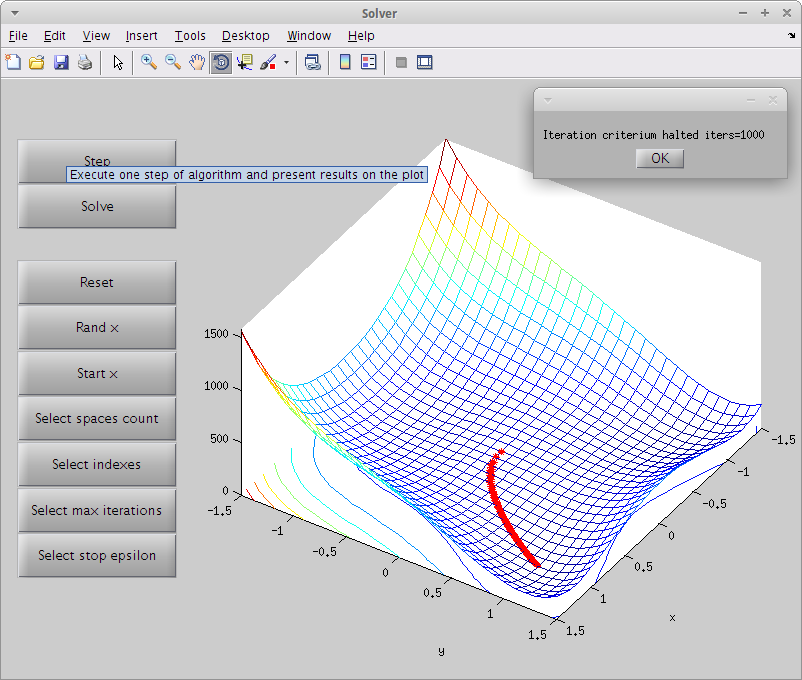
\includegraphics[height=13cm]{../res/img/gui_snap_solve.png}
    \end{center}
    \caption{GUI aplikacji}\label{img:gui1}
\end{figure}

\newpage

Do kontroli przebiegu algorytmu użyte są następujące przyciski:

\begin{itemize}
  \item ,,Step'' - wylicza jeden kolejny punkt przybliżający minimum i wyświetla
  go na wykresie
  \item ,,Solve'' - wylicza kolejne przybliżenia minimum, aż do zadziałania
  jednego z kryteriów stopu
  \item ,,Reset'' - przywraca stan algorytmu do punktu początkowego
  \item ,,Rand x'' - losuje punkt początkowy i przywraca stan algorytmu do
  punktu początkowego
  \item ,,Start x'' - wyświetla okienko pozwalające podać punkt początkowy i
  przywraca stan algorytmu do punktu początkowego
  \item ,,Select spaces count'' - wyświetla okienko pozwalające podać liczbę
  wymiarów do analizy
  \item ,,Select max iterations'' - wyświetla okienko pozwalające ograniczyć
  maksymalną liczbę iteracji algorytmu w przypadku użycia opcji
  ,,Solve''(pierwsze kryterium stopu)
  \item ,,Select stop epsilon'' - pozwala wybrać minimalny spadek wartości
  funkcji który nie spowoduje zatrzymania algorytmu w przypadku użycia opcji
  ,,Solve''(drugie kryterium stopu)
\end{itemize}


\end{document}